\documentclass[10pt,twocolumn,letterpaper]{article}

\usepackage{cvpr}
\usepackage{times}
\usepackage{epsfig}
\usepackage{graphicx}
\usepackage{amsmath}
\usepackage{amssymb}

% Include other packages here, before hyperref.

% If you comment hyperref and then uncomment it, you should delete
% egpaper.aux before re-running latex.  (Or just hit 'q' on the first latex
% run, let it finish, and you should be clear).
\usepackage[breaklinks=true,bookmarks=false]{hyperref}

\cvprfinalcopy % *** Uncomment this line for the final submission

\def\cvprPaperID{****} % *** Enter the CVPR Paper ID here
\def\httilde{\mbox{\tt\raisebox{-.5ex}{\symbol{126}}}}

% Pages are numbered in submission mode, and unnumbered in camera-ready
%\ifcvprfinal\pagestyle{empty}\fi
\setcounter{page}{1}
\begin{document}

%%%%%%%%% TITLE
\title{ Computer Vision Lab SS16\\ P-CNN: Pose-based CNN Features for Action Recognition}

\author{Ahmed Abdelbaki\\
University of Bonn\\
Bonn, Germany\\
{\tt\small abdelbak@iai.uni-bonn.de}
}

\maketitle
%\thispagestyle{empty}

%%%%%%%%% ABSTRACT
\begin{abstract}
   This work targets human action recognition in video based on the state of art deep convolutional neural network (CNN). Recent methods represents actions by statistics of local video features,here we argue for the importance of a representation derived from human pose. We are using an approach called Pose-based Convolutional Neural Network descriptor (P-CNN) for action recognition. The descriptor aggregates motion and appearance information through patches of human body parts. We investigate different CNN model fro the P-CNN approach and experiment P-CNN features obtained  both for automatically estimated and manually annotated human poses. We evaluate our method on the recent and challenging JHMDB dataset. Our evaluation shows consistent improvement over the original approach.
   
\end{abstract}

%%%%%%%%% BODY TEXT
\section{Introduction}

Recognition of human actions is an important step toward
fully automatic understanding of dynamic scenes. Despite
significant progress in recent years, action recognition
remains a difficult challenge. Common problems stem from
the strong variations of people and scenes in motion and appearance.
Other factors include subtle differences of fine-grained
actions, for example when manipulating small objects
or assessing the quality of sports actions.\\

The majority of recent methods recognize actions based
on statistical representations of local motion descriptors
\cite{schuldt2004recognizing,laptev2008learning,wang2013action}. These approaches are very successful
in recognizing coarse action (standing up, hand-shaking,
dancing) in challenging scenes with camera motions, occlusions,
multiple people, etc. Global approaches, however,
are lacking structure and may not be optimal to recognize
subtle variations, e.g. to distinguish correct and incorrect
golf swings or to recognize fine-grained cooking actions 

In this work, we are using the P-CNN approach which is a new action descriptor based on human poses. Provided with tracks of body joints over time,it combines motion and appearance features for
body parts. In \cite{cheron2015p}, they explore CNN features obtained
separately for each body part in each frame due to the recent success of CNN \cite{krizhevsky2012imagenet,lecun1998gradient}. We use
appearance and motion-based CNN features computed for each track of body parts and investigate different patch extraction mechanisms which are based on human joints pose. Moreover, we examine different CNN architecture for the feature extraction by comparing between the "VGG-F" Net \cite{chatfield2014return} and Microsoft Residual Networks(ResNet) \cite{he2015deep}. The CNN features extraction pipeline of (P-CNN) is illustrated in figure \ref{fig:pcnn}.

The rest of the paper/technical report is organized as follows. Related work is discussed in Section\ref{related-work}. Section\ref{pcnn-features} introduces the P-CNN approach and CNN features extraction. Our contribution of the improved P-CNN is explained in Section\ref{ipcnn}. We present the Dataset used in our experiments in Section\ref{dataset} and summarize the experimental results in Section\ref{results}.

\begin{figure*}
	\begin{center}
		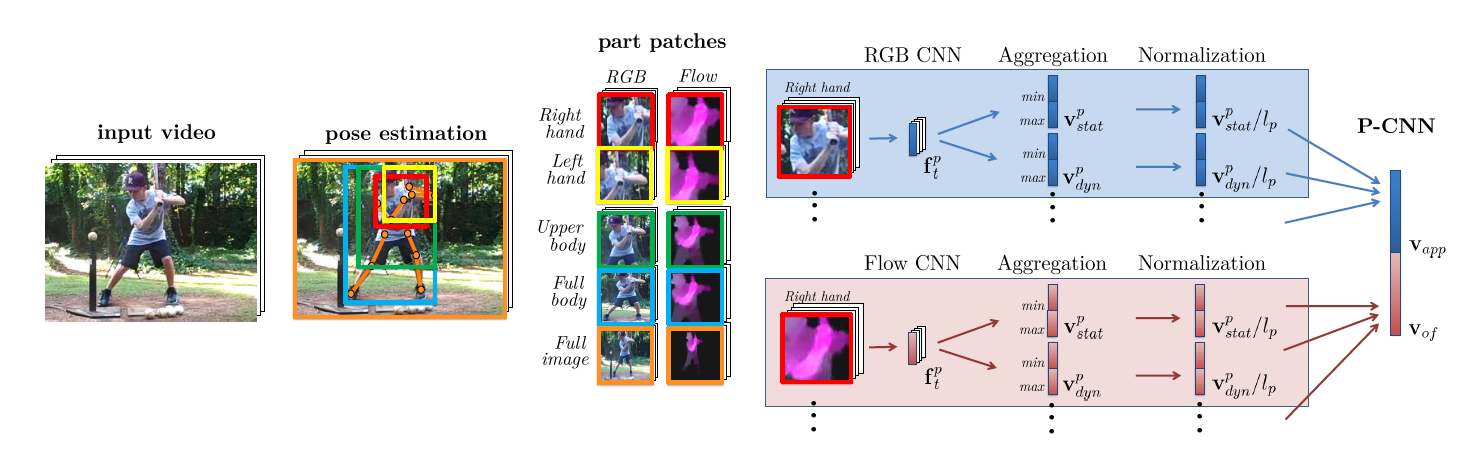
\includegraphics[width=1.0\linewidth]{P-CNN}
	\end{center}
	\caption{P-CNN features. From left to right: Input video. Human pose and corresponding human body parts for one frame
		of the video. Patches of appearance (RGB) and optical flow for human body parts. One RGB and one flow CNN descriptor $f^{p}_{t}$ is extracted per frame \textit{t} and per part \textit{p} (an example is shown for the human body part \textit{right hand}). Static frame descriptors $f^{p}_{t}$ are aggregated over time using \textit{min} and \textit{max} to obtain the video descriptor $v^{p}_{stat}$. Similarly, temporal differences of $f^{p}_{t}$ are aggregated to $v^{p}_{dyn}$. Video descriptors are normalized and concatenated over parts \textit{p} and aggregation schemes into appearance features $v_{app}$ and flow features $v_{of}$. The final P-CNN feature is the concatenation of $v_{app}$ and $v_{of}$. }
	\label{fig:pcnn}
\end{figure*}

\section{Related work}
\label{related-work}
Action Recognition in the last decade has been dominated by local and hand crafted features. In particular, Dense Trajectories (DT) features\cite{wang2013action} combined with Fisher Vector (FV)\cite{perronnin2010improving} aggregation have shown magnificent results for many challenging benchmarks.

The latest breakthroughs in Convolutional Neural Networks (CNN) have impacted a significant progress in image classification and other vision tasks.Although the applications of CNNs to action recognition in video\cite{simonyan2014two,yue2015beyond} has shown only limited improvements so far. P-CNN approach extend previous global CNN methods and address action recognition using CNN descriptors at the local level of human body parts.

Most of the recent methods for action recognition deploy global aggregation of local video descriptors. Such representations provide invariance to numerous variations
in the video but may fail to capture important spatio-temporal structure. For fine-grained action recognition, previous methods represented person-object interactions by joint tracking of hands and objects\cite{ni2014multiple} or, by linking
object proposals\cite{zhou2015interaction}. Alternative methods represent action using positions and temporal difference of body joints. Hence, it seems that Pose Estimation is a very important task for action recognition;however, reliable human pose estimation is still a challenging task. A recent study \cite{jhuang2013towards} reports significant gains provided by dynamic human pose features in case of the availability of reliable pose estimation. P-CNN extend the work \cite{jhuang2013towards} and designed a new CNN-based representation for human actions combing positions, appearance and motion of human joints.

\section{P-CNN: Pose-based CNN features}
\label{pcnn-features}
\noindent
Compare the following:\\
\begin{tabular}{ll}
 \verb'$conf_a$' &  $conf_a$ \\
 \verb'$\mathit{conf}_a$' & $\mathit{conf}_a$
\end{tabular}\\
See The \TeX book, p165.

The space after \eg, meaning ``for example'', should not be a
sentence-ending space. So \eg is correct, {\em e.g.} is not.  The provided
\verb'\eg' macro takes care of this.

When citing a multi-author paper, you may save space by using ``et alia'',
shortened to ``\etal'' (not ``{\em et.\ al.}'' as ``{\em et}'' is a complete word.)
However, use it only when there are three or more authors.  Thus, the
following is correct: ``
   Frobnication has been trendy lately.
   It was introduced by Alpher~\cite{Alpher02}, and subsequently developed by
   Alpher and Fotheringham-Smythe~\cite{Alpher03}, and Alpher \etal~\cite{Alpher04}.''

This is incorrect: ``... subsequently developed by Alpher \etal~\cite{Alpher03} ...''
because reference~\cite{Alpher03} has just two authors.  If you use the
\verb'\etal' macro provided, then you need not worry about double periods
when used at the end of a sentence as in Alpher \etal.

For this citation style, keep multiple citations in numerical (not
chronological) order, so prefer \cite{Alpher03,Alpher02,Authors13} to
\cite{Alpher02,Alpher03,Authors13}.




%------------------------------------------------------------------------
\section{IPCNN: Improved P-CNN}
\label{ipcnn}
All text must be in a two-column format. The total allowable width of the
text area is $6\frac78$ inches (17.5 cm) wide by $8\frac78$ inches (22.54
cm) high. Columns are to be $3\frac14$ inches (8.25 cm) wide, with a
$\frac{5}{16}$ inch (0.8 cm) space between them. The main title (on the
first page) should begin 1.0 inch (2.54 cm) from the top edge of the
page. The second and following pages should begin 1.0 inch (2.54 cm) from
the top edge. On all pages, the bottom margin should be 1-1/8 inches (2.86
cm) from the bottom edge of the page for $8.5 \times 11$-inch paper; for A4
paper, approximately 1-5/8 inches (4.13 cm) from the bottom edge of the
page.

%-------------------------------------------------------------------------
\section{Datasets}
\label{dataset}
In our experiments, we use a well-known dataset called JHMDB (Joint-annotated Human Motion Data Base)\cite{jhuang2013towards}. We present it in the following.
\paragraph{JHMDB}is a subset of \textbf{HMDB}\cite{kuehne2011hmdb}, see figure \ref{fig:JHMDB}. It contains 21 human actions, such as \textit{brush hair, climb, golf, run or sit}. Video clips are restricted to the duration of the action. There are between 36 and 55 clips per action
for a total of 928 clips. Each clip contains between 15 and
40 frames of size 320 X 240. Human pose is annotated in each of the 31838 frames. There are 3 train/test splits for the JHMDB dataset and evaluation averages the results over these three splits. The metric used is accuracy: each clip
is assigned an action label corresponding to the maximum value among the scores returned by the action classifiers.

\begin{figure}
	\begin{center}
		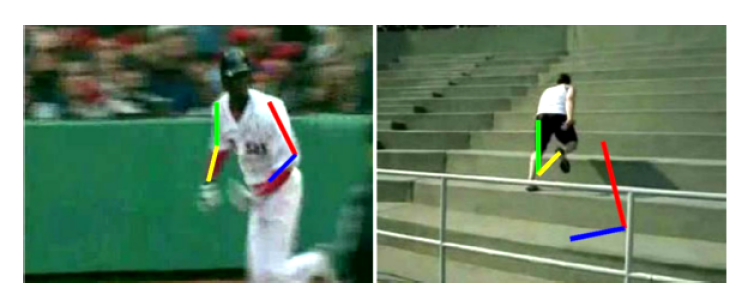
\includegraphics[width=1.0\linewidth]{JHMDB}
	\end{center}
	\caption{Examples from JHMDB dataset}
	\label{fig:JHMDB}
\end{figure}


%-------------------------------------------------------------------------
\section{Experimental results}
\label{results}
Wherever Times is specified, Times Roman may also be used. If neither is
available on your word processor, please use the font closest in
appearance to Times to which you have access.

MAIN TITLE. Center the title 1-3/8 inches (3.49 cm) from the top edge of
the first page. The title should be in Times 14-point, boldface type.
Capitalize the first letter of nouns, pronouns, verbs, adjectives, and
adverbs; do not capitalize articles, coordinate conjunctions, or
prepositions (unless the title begins with such a word). Leave two blank
lines after the title.

AUTHOR NAME(s) and AFFILIATION(s) are to be centered beneath the title
and printed in Times 12-point, non-boldface type. This information is to
be followed by two blank lines.

The ABSTRACT and MAIN TEXT are to be in a two-column format.

MAIN TEXT. Type main text in 10-point Times, single-spaced. Do NOT use
double-spacing. All paragraphs should be indented 1 pica (approx. 1/6
inch or 0.422 cm). Make sure your text is fully justified---that is,
flush left and flush right. Please do not place any additional blank
lines between paragraphs.

Figure and table captions should be 9-point Roman type as in
Figures~\ref{fig:onecol} and~\ref{fig:short}.  Short captions should be centred.

\noindent Callouts should be 9-point Helvetica, non-boldface type.
Initially capitalize only the first word of section titles and first-,
second-, and third-order headings.

FIRST-ORDER HEADINGS. (For example, {\large \bf 1. Introduction})
should be Times 12-point boldface, initially capitalized, flush left,
with one blank line before, and one blank line after.

SECOND-ORDER HEADINGS. (For example, { \bf 1.1. Database elements})
should be Times 11-point boldface, initially capitalized, flush left,
with one blank line before, and one after. If you require a third-order
heading (we discourage it), use 10-point Times, boldface, initially
capitalized, flush left, preceded by one blank line, followed by a period
and your text on the same line.

%-------------------------------------------------------------------------
\subsection{Footnotes}

Please use footnotes\footnote {This is what a footnote looks like.  It
often distracts the reader from the main flow of the argument.} sparingly.
Indeed, try to avoid footnotes altogether and include necessary peripheral
observations in
the text (within parentheses, if you prefer, as in this sentence).  If you
wish to use a footnote, place it at the bottom of the column on the page on
which it is referenced. Use Times 8-point type, single-spaced.


%-------------------------------------------------------------------------
\subsection{References}

List and number all bibliographical references in 9-point Times,
single-spaced, at the end of your paper. When referenced in the text,
enclose the citation number in square brackets, for
example~\cite{Authors13}.  Where appropriate, include the name(s) of
editors of referenced books.

\begin{table}
\begin{center}
\begin{tabular}{|l|c|}
\hline
Method & Frobnability \\
\hline\hline
Theirs & Frumpy \\
Yours & Frobbly \\
Ours & Makes one's heart Frob\\
\hline
\end{tabular}
\end{center}
\caption{Results.   Ours is better.}
\end{table}

%-------------------------------------------------------------------------
\subsection{Illustrations, graphs, and photographs}

All graphics should be centered.  Please ensure that any point you wish to
make is resolvable in a printed copy of the paper.  Resize fonts in figures
to match the font in the body text, and choose line widths which render
effectively in print.  Many readers (and reviewers), even of an electronic
copy, will choose to print your paper in order to read it.  You cannot
insist that they do otherwise, and therefore must not assume that they can
zoom in to see tiny details on a graphic.

When placing figures in \LaTeX, it's almost always best to use
\verb+\includegraphics+, and to specify the  figure width as a multiple of
the line width as in the example below
{\small\begin{verbatim}
   \usepackage[dvips]{graphicx} ...
   \includegraphics[width=0.8\linewidth]
                   {myfile.eps}
\end{verbatim}
}





{\small
\bibliographystyle{ieee}
\bibliography{egbib}
}

\end{document}
